\subsection{Message showing procedure}

%%//poner fotos 4-digit 7-segment display//
With respect to the layout of the numbers and messages, a single 7-segment display followed by a 4-digit 7-segment Common Anode display are needed. 
Regarding the 7-segment display, it has integrated a decoder, which translates the BCD directly to its representation into the display.

\medskip

The 4-digit 7-segment display has an input for each of the segments, meaning that you can command the functioning of each segment. Another 4 terminals select which of the 4 displays are functioning. In order to show all four displays at a time, either the password or OPEN/ERROR messages, a high frequency ring is needed.

\medskip

In order to be able to deal with the data coming from different GALs, tristate buffers are necessary. Due to the fact that there is a GAL that whose purpose is to choose which of the messages is going to be displayed, this is, showing a high state depending on the message. 

\medskip

This high state, is used as an enabling signal for the tristates buffers, some for the message itself and others for the ring signal. 

%% poner foto subsystema 

Regarding the functioning of the display, there will be a tristate buffer for each of the segments, as well as for each of the messages, depending on the shape of each of the characters, a HIGH or LOW level will be applied. However, the tristates buffers that control the ring signal have at the input the ring signal provided by each of the GALs.

\begin{figure}[H]
    \centering
    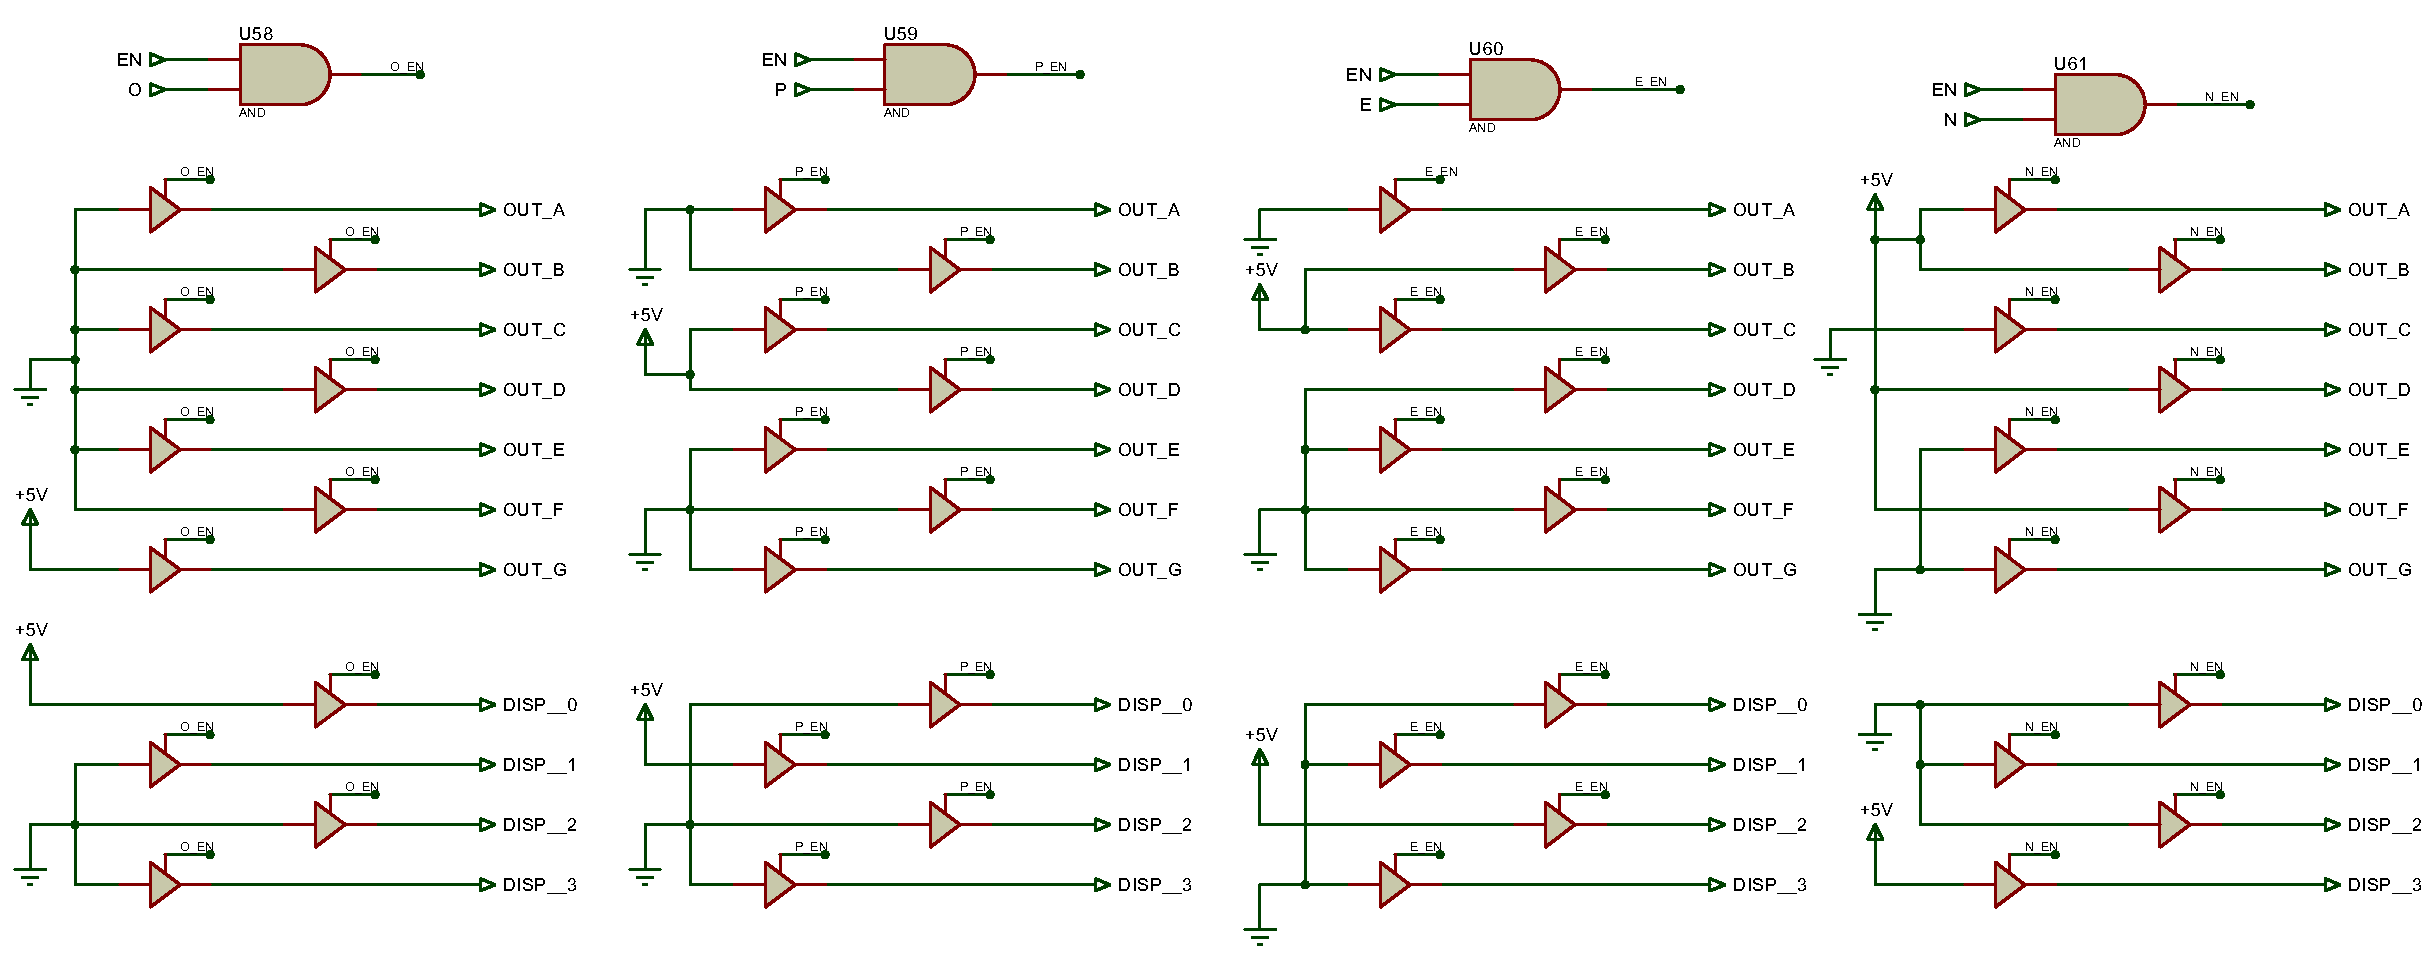
\includegraphics[scale = 0.35]{Graphics/MESSAGE/OPEN.PDF}
    \caption{OPEN message}
    \label{fig:OPEN_MESSAGE}
\end{figure}



